\begin{document}
	
	\chapter{Invatare automata}
	
		\begin{center}
		"Orice aspect al invatarii sau caracteristica a inteligentei poate fi descrisa atat de precis incat o masina poate fi facuta sa o simuleze"\cite{mccarthy_proposal} 
		\end{center}
	
	Invatarea este definita ca fiind achizitia cunostiintelor sau a aptitudinilor prin studiu, experienta sau prin invatare. Definitia acopera intr-un mod minimal modalitatea de functionare a invatarii automate in randul sistemelor. Pentru a putea fi cababili de a invata o masina cum sa ia decizii intr-un mod asemanator creierului uman, este necesara intelegerea gandirii umane. Acest lucru poate fi realizat prin introspectie sau prin experimente psihologice.  
	Fundamente de baza ale invatarii automate pot fi regasite de asemenea in comportamentul si abilitatea de invatare a animalelor. Un exemplu concret ar fi modul in care sobolanii reactioneaza la hrana cu miros sau aspect nefamiliar. Acestia vor lua cantitati mici din hrana la inceput, iar bazat pe gust si efectul asupra lor, vor lua progresiv cantitati mai mari. Daca hrana are un efect negativ asupra sobolanilor, nu doar ca nu o vor manca dar vor folosi experienta in viitor cand vor fi pusi din nou in fata unui miros sau aspect nefamiliar, evitand hrana. 
	
	\section{Aspecte generale}
	Abilitatea sistemelor de a lua decizii fara o indrumare explicita a fost o provocare pentru multe domenii stiintifice, iar procesul de descoperire este inca in derulare, avand un progres vizibil in ziua de astazi. La baza acestei capabilitati ale sistemelor, se afla algoritmi construiti si optimizati pe parcusul istoriei, sustinuti de avansarea tehnologiei si cresterea semnificativa a masei de informatie si a valabilitatii ei. 
	Algoritmii au urmarit mai multe tipologii, care astazi se rezuma la doi: invatare supervizata si invatare nesupervizata. Desi algoritmii invatarii automata difera de la unul la celalalt, scopul lor este comun.
	
	\subsection{Puncte cheie in istoria intelgentei artificiale}
	In prima jumatate a secolului 20 filmele science fiction au adus in lumina inteligenta artificiala prin intermediul a mai multor personaje. Printre primele personaje care sustineau acest concept a fost Tin, omul de tinichea, din vrajitorul din Oz, care a fost urmat la scurt timp de robotul cu caracter uman, Maria, din “Metropolis”. Prezenta acestor personaje scoate in evidenta interesul, chiar daca involuntar, a oamenilor in abilitatea unor sisteme de a prelua comportamentul celui mai complex lucru din lume pana in momentul de fata, creierul uman. 
	
	Pana in anii 50 lumea s-a bucurat de o generatie de cercetatori in stiinta, matematica si filozofie care aveau un tel comun, si anume, aducerea din filme si fictiune a “sistemelor inteligente” la realitate. Printre acele persoane se enumara si Alan Turing, o personalitate remarcabila in IT-ul de astazi de care lumea se bucura si profita. Turing a folosit o interpretare matematica pentru a demonstra posibilitatea de existenta a inteligentei masinariilor,un domeniu nedefinit la momentul acela. Acesta era de parere ca daca oamenii pot rezolva o problema utilizand un motiv si informatii, un calculator ar putea sa faca la fel. \cite{ai_history}
	
	In 1950, Alan Turing vine cu o lucrare care va avea sa incepea cu fraza “Can machines think?”. Lucrarea va avea sa puna bazele metodelor prin care masinile inteligente sunt construite si testate. Acesta face o analogie, in lucrarea sa, intre inteligenta artificiala si un joc pe care acesta il numeste “The Imitation Game”, care este alcatuit din 3 jucatori: Un barbat, reprezentat prin A, o femeie, reprezentata prin B, si un interogator. Interogatorul sta intr-o alta camera decat barbatul si femeia. Scopul interogatorului este sa isi dea seama, pana la finalul jocului, care dintre A si B este femeia si care este barbatul. Acesta poate pune intrebari fiecaruia, in scopul de a-si da seama din descriere genul persoanei intrebate. Intrebarea va fi pusa atunci cand un calculator va lua locul lui A sau B. Va creste nivelul dificultatii pentru interogator ? Alan Turing si-a sustinut intrebarea de la inceputul  articolului prin aceasta analogie. \cite{turing}
	
	In 1955, avea sa fie conturat acest domeniu, al masinilor inteligente, pentru prima data, de catre omul de stiinta John McCarthy, recunoscut in zilele de astazi, ca si fiind tatal inteligentei artificiale. Acesta a inventat si a definit domeniul inteligentei artificiale, prin propunerea sa de lucrarea, la conferinta ce a avut loc in anul 1956 la Dartmouth. Lucrarea sa urmarea sa exploreze posibilitatile de intelegere, invatare si auto-dezvoltare a unei masini. Acesta considera ca orice act de inteligenta a omului este studiat si  inteles la un nivel atat de ridicat,  incat ar putea fi transpus in rutina calculatoarelor. Anul 1958, John McCarthy creeaza limbajul de programare LISP, care va deveni limbajul de baza a inteligentei artificiale si va avea sa ramana astfel pana in zilele de astazi. [5]
	John McCarthy a pus bazele unui domeniu care este studiat intensiv si in momentul actual si care nu are un progres liniar si predictiv. Acesta considera, la acel moment, ca apogeul inteligentei artificiale ar putea aparea in 5 ani, sau ar putea aparea in 500 de ani, dar nu a negat niciodata posibilitatea de dezvoltare si avansare a acestui domeniu.
	
	
	\subsection{Cum functioneaza?}
	Invatarea automata urmareste un sablon (Figura 1.), a carui scop este dezvoltarea unui model capabil de a separa datele de intrare, in grupuri care au aspecte comune, astfel putand sa le clasifice. Datele de intrare sunt adesea distribuite in asa fel incat trasarea unei linii drepte in plan nu va putea clasifica corect datele, astfel  modelul va trebui sa gaseasca o corelatie neliniara intre datele care ii sunt date si rezultatul care va servi ca predictie a sa. (Vezi Figura \ref{fig:uml-diagram})
	
	\vfill
	
	\begin{figure}[H]
		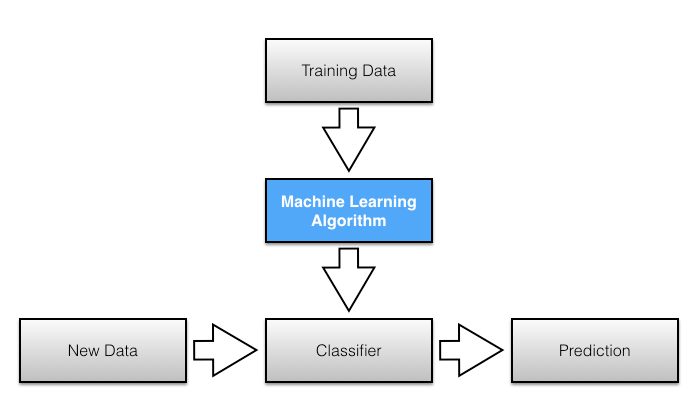
\includegraphics[width=15cm]{ml-uml}  
		\caption{\label{fig:uml-diagram} Diagrama generala a algoritmului de invatare supervizata \cite{predictive_modelling}}
	\end{figure}
	
\end{document}